\documentclass[12pt, a4paper]{article} 
 
\usepackage[utf8]{inputenc}
 
 
\usepackage{geometry} % to change the page dimensions
\geometry{a4paper} % or letterpaper (US) or a5paper or....
 
\usepackage{graphicx} % support the \includegraphics command and options
 
\usepackage{booktabs} % for much better looking tables
\usepackage{array} % for better arrays (eg matrices) in maths
\usepackage{paralist} % very flexible & customisable lists (eg. enumerate/itemize, etc.)
\usepackage{verbatim} % adds environment for commenting out blocks of text & for better verbatim
\usepackage{subfig} % make it possible to include more than one captioned figure/table in a single float
% These packages are all incorporated in the memoir class to one degree or another...
 
 
 
\usepackage{amsmath, amssymb}% for mathematical symbols
\usepackage[colorlinks=true,linkcolor=black, urlcolor=blue]{hyperref} % for hyperreferences with black color
%\usepackage[T1]{fontenc} % Uncomment for norwegian document
%\usepackage[norsk]{babel} %
 
%%% HEADERS & FOOTERS
\usepackage{fancyhdr} % This should be set AFTER setting up the page geometry
\pagestyle{fancy} % options: empty , plain , fancy
\renewcommand{\headrulewidth}{0pt} % customise the layout...
\lhead{}\chead{}\rhead{}
\lfoot{}\cfoot{\thepage}\rfoot{}
 
%%% SECTION TITLE APPEARANCE
\usepackage{sectsty}
\allsectionsfont{\sffamily\mdseries\upshape} % (See the fntguide.pdf for font help)
% (This matches ConTeXt defaults)
 
%%% ToC (table of contents) APPEARANCE
\usepackage[nottoc,notlof,notlot]{tocbibind} % Put the bibliography in the ToC
\usepackage[titles,subfigure]{tocloft} % Alter the style of the Table of Contents
\renewcommand{\cftsecfont}{\rmfamily\mdseries\upshape}
\renewcommand{\cftsecpagefont}{\rmfamily\mdseries\upshape} % No bold!

\begin{document}

\section{Architecture}

\subsection{Stakeholders}

\subsubsection{Customer}
Our goal with this course is to make a product that work as the customer intended but also performs satisfactorily. The code we're writing needs to be written following the clean coding standard and use interfaces/polymorphy so their developers can further develop this solution.

\subsubsection{Course Evaluator}
The course evaluator needs to be satisfied if we want a good grade, that means that we need to satisfy all the other stakeholders and deliver a well documented report of everything.

\subsubsection{Supervisor}
The supervisor said in the first meeting that he would fight for our grade given that he was satisfied. This means that we should complete the project deliver a well documented report. \\ We should also take advices from him, especially when there's issues among us in which we need to tell the supervisor so he can help solve the issue.
\subsubsection{Implementers}
The architecture should be easy to implement and make sense to the coders.

\subsection{Quality Attributes}
The customer was very specific when it came to what they wanted.
\subsubsection{Modifiability}
The solution we're making will be used for other ads than real estate ads, therefore we need to make it modifiable so other developers later on can further develop using our solution as a base.
\subsubsection{Performance}
We want the system to perform with a satisfactory performance.
\subsubsection{Availability}
The system should be available for the users when they need it.
\subsubsection{Interoperability}
Needs to inter-operate with already-existing order system, this will be done by using the technology the customer tells us to use; Web-api, mssql etc...

\subsection{Views}

\subsubsection{Logical view}
\begin{figure}[h]
\centering
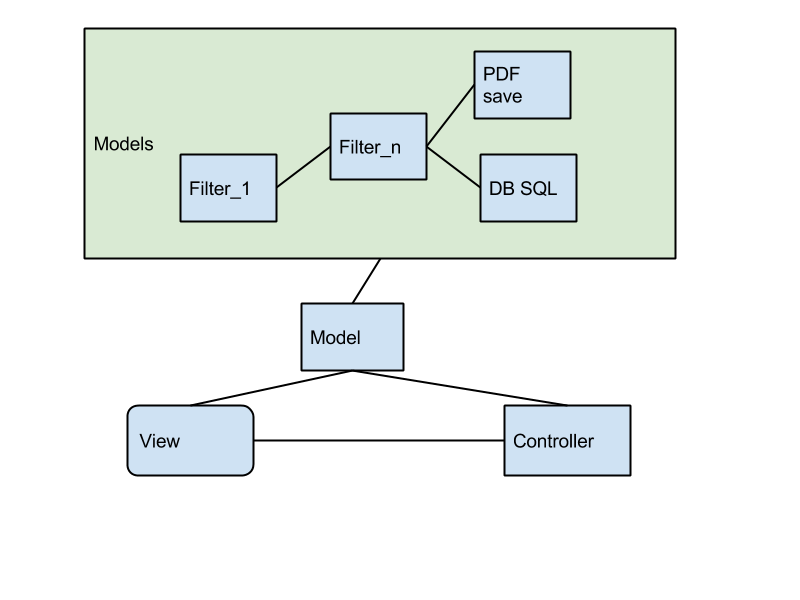
\includegraphics[width=0.8\textwidth]{images/architecture00.png}
\caption{Logical view}
\label{fig:logical_view}
\end{figure}
\subsubsection{Process view}
\newpage
\subsubsection{Scenario view}
\begin{figure}[h]
\centering
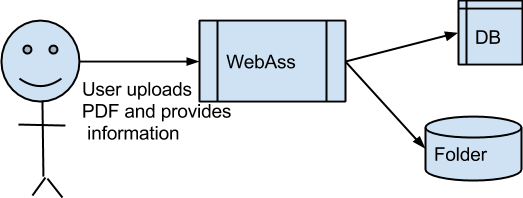
\includegraphics[width=0.8\textwidth]{images/architecture01.png}
\caption{Scenario view}
\label{fig:scenario_view}
\end{figure}



\subsubsection{Physical view}
\begin{figure}[h]
\centering
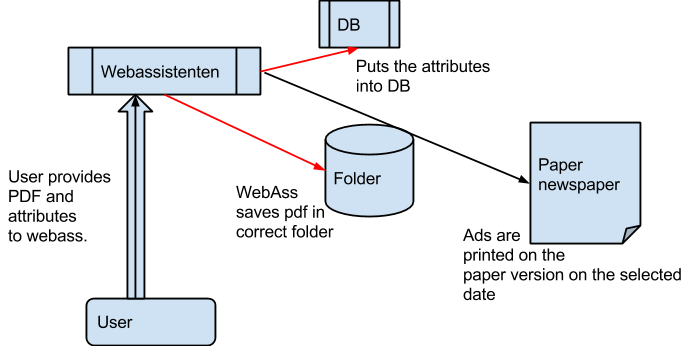
\includegraphics[width=0.8\textwidth]{images/architecture02.png}
\caption{Physical view, we implement the red arrows}
\label{fig:physical_view}
\end{figure}

\subsection{Patterns}
MVC due to the technology and pipe \&  filter to filter the data and due to the modifiability requirement.
\subsection{Tactics}
\subsubsection{Modifiability}
\begin{itemize}
\item Increase semantic cohesion
\item Decrease coupling
\item Split modules
\end{itemize}

\subsubsection{Performance}
\begin{itemize}
\item Write optimal code
\end{itemize}

\subsubsection{Availability}
\begin{itemize}
\item Our code should not crash the customer's system, but it's their responsibility that the system is available.
\end{itemize}

\subsubsection{Interoperability}
\begin{itemize}
\item The technology and tools we're using should be sufficient to ensure interoperability
\end{itemize}

\end{document}